\documentclass[a4paper]{article}

\usepackage[text={18.6cm, 26.0cm}, centering]{geometry}

\usepackage[czech, provide=*]{babel}
\usepackage[utf8]{inputenc}
\usepackage[T1]{fontenc}
\usepackage{color}
\usepackage{alltt} % \verb
\usepackage[hidelinks]{hyperref} % odkazy
\usepackage{tikz}

% Ceske uvozovky
\providecommand{\uv}[1]{\quotedblbase #1\textquotedblleft}

\begin{document}
    \begin{titlepage}
        \begin{center}
            \textsc{\Huge{}Vysoké učení technické v Brně\\[0.5em]}
            \textsc{\huge Fakulta informačních technologií}\\
            \vspace{\stretch{0.382}}
            { \huge Wren překladač\,--\,dokumentace\\[0.5em]
                IFJ/IAL 2025 }\\[0.5em]
                Tým xsebesm00, varianta TRP-izp\\
            \vspace{\stretch{0.618}}
        \end{center}
        { \phantom{a}\hfill FUNEXP\\
          \phantom{a}\hfill EXTSTAT\\
          Vojtěch Borýsek (xborysv00)\,--\, 33\% \hfill EXTFUN\\
          Šimon Halas (xhalass00)\,--\, 00\% \hfill BOOLTHEN\\
          Tomáš Hanák (xhanakt00)\,--\, 33\% \hfill OPERATORS\\
          Michal Šebesta (xsebesm00)\,--\, 34\%, vedoucí \hfill STATICAN\\
          }
    \end{titlepage}
    \tableofcontents
    \newpage
    \section{Přehled}
        \begin{center}
            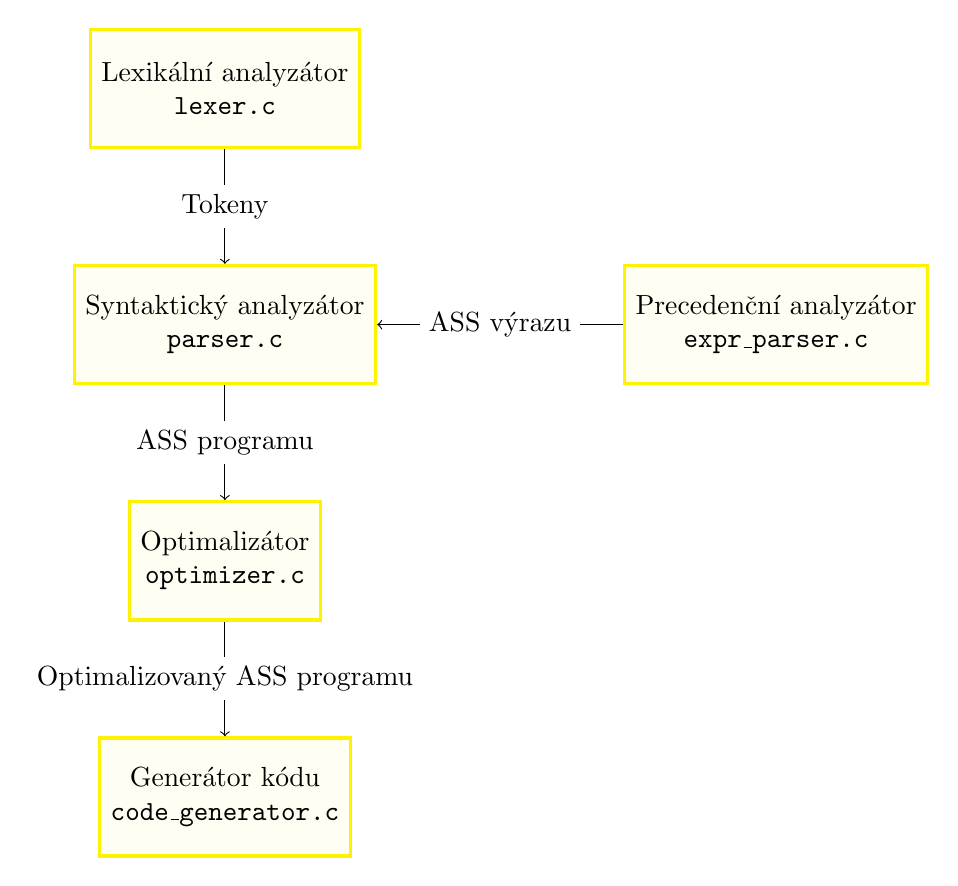
\begin{tikzpicture}[
                    every node/.style={fill=white},
                    block/.style={rectangle, draw=yellow, fill=yellow!5, very thick, minimum size=15mm, inner sep=4pt,draw},
                    node distance=3cm,
                    align=center,
                ]
                \node[block] (lexer) {Lexikální analyzátor\\ \texttt{lexer.c}};
                \node[block] (parser) [below of=lexer] {Syntaktický analyzátor\\ \texttt{parser.c}};
                \node[block] (expr) [right of=parser, xshift=4cm]{Precedenční analyzátor\\ \texttt{expr\_parser.c}};
                \node[block] (optimizer) [below of=parser] {Optimalizátor\\ \texttt{optimizer.c}};
                \node[block] (codegen) [below of=optimizer] {Generátor kódu\\ \texttt{code\_generator.c}};

                \draw[->] (lexer.south) -- node {Tokeny} (parser.north);
                \draw[->] (expr.west) -- node {ASS výrazu} (parser.east);
                \draw[->] (parser.south) -- node {ASS programu} (optimizer.north);
                \draw[->] (optimizer.south) -- node {Optimalizovaný ASS programu} (codegen.north);
            \end{tikzpicture}
        \end{center}
        Překlad začíná inicializací lexikálního analyzátoru. Ten je následně předán syntaktickému analyzátoru,
        který jej volá v případě potřeby tokenu. Pokud syntaktický analyzátor potřebuje načíst výraz, volá precedenční
        analyzátor. V rámci syntaktického analyzátoru se rovnou také provádí sémantické akce,
        jako kontrola typů výrazů, nebo kontrola deklarace proměnných. Výsledek ukládá do abstraktního
        syntaktického stromu (ASS).

        Jakmile je celý program převeden na ASS a sémanticky zkontrolován, je tento strom předán do optimalizátoru, který strom zoptimalizuje.
        Optimalizovaný strom je následně předán generátoru kódu, který z něj vytvoří cílový kód, čímž překlad končí.


    \section{Lexikální analýza}
        TODO

    \section{Syntaktický analýza}
        TODO
    \subsection{Tabulka symbolů}
        TODO
    \subsection{Sémantická analýza}
        TODO
    \subsection{Zpracování výrazů}
        TODO
    \subsection{Abstraktní syntaktický strom}
        TODO

    \section{Optimalizátor}
        TODO

    \section{Generátor kódu}
        TODO

    \section{Rozdělení práce}
        \textbf{Vojtěch Borýsek}: Implementace precedenční analýzy a datových struktur.\\
        \textbf{Šimon Halas}: Implementace tabulky symbolů. Hodnocení 0\% kvůli plánovanému ukončení studia.\\
        \textbf{Tomáš Hanák}: Implementace syntaktické a sémantické analýzy a optimalizátoru.\\
        \textbf{Michal Šebesta}: Implementace lexikálního analyzátoru a generátoru kódu.
\end{document}
